\subsection{Zernike modes PSFs Clustering}

	\subsubsection{UMAPS}
		
		Before clustering, UMAPS for flattened PSF matrices, flattend LP coefficients matrices and PL intensities are processed. The same configuration is used for the different number of modes.
		
		\begin{table}[h!]
			\centering
			\begin{tabular}{|c|c|c|c|}
				\hline
				\textbf{Dataset type} & \textbf{Number of neighbors} & \textbf{Min distance} & \textbf{Number of components} \\
				\hline
				Zernike modes PSF & 500 & 0.3 & 3 \\
				\hline
				LP coefficients & 500 & 0.1 & 2 \\
				\hline
				PL intensities & 500 & 0.1 & 2 \\
				
				\hline
			\end{tabular}
		\caption{UMAP parameter configurations for each of the dataset type}
		\end{table}
		
		The resulting projections are the following:
		\begin{figure*}[ht!]
			\centering
			\subfloat[2 Zernike modes LP coefficients UMAP]{%
			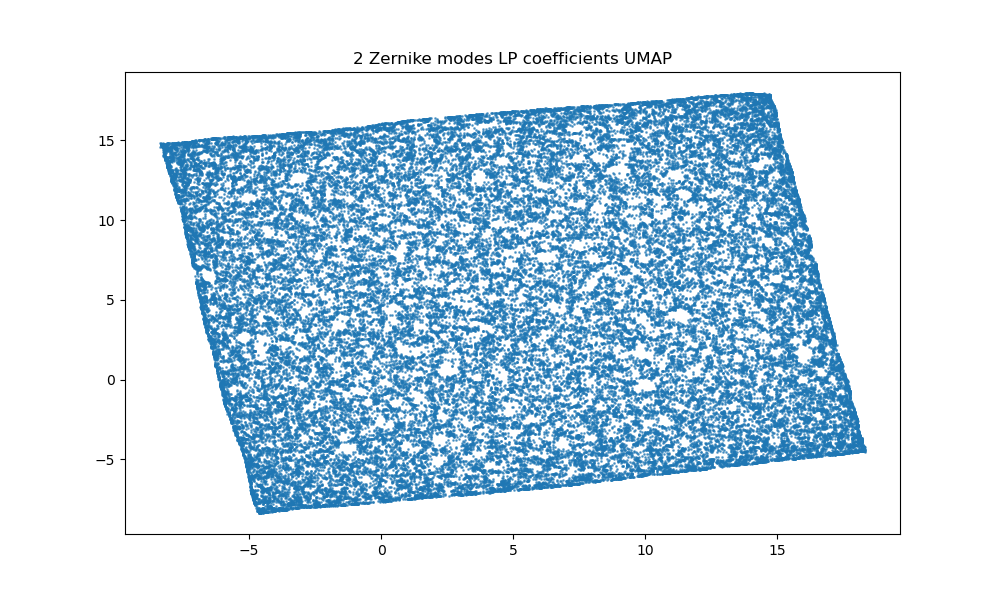
\includegraphics[ width=0.31\textwidth]{pid-2mlpumap.png}}
			\hspace{\fill}
			\subfloat[2 Zernike modes PL intensities UMAP]{%
			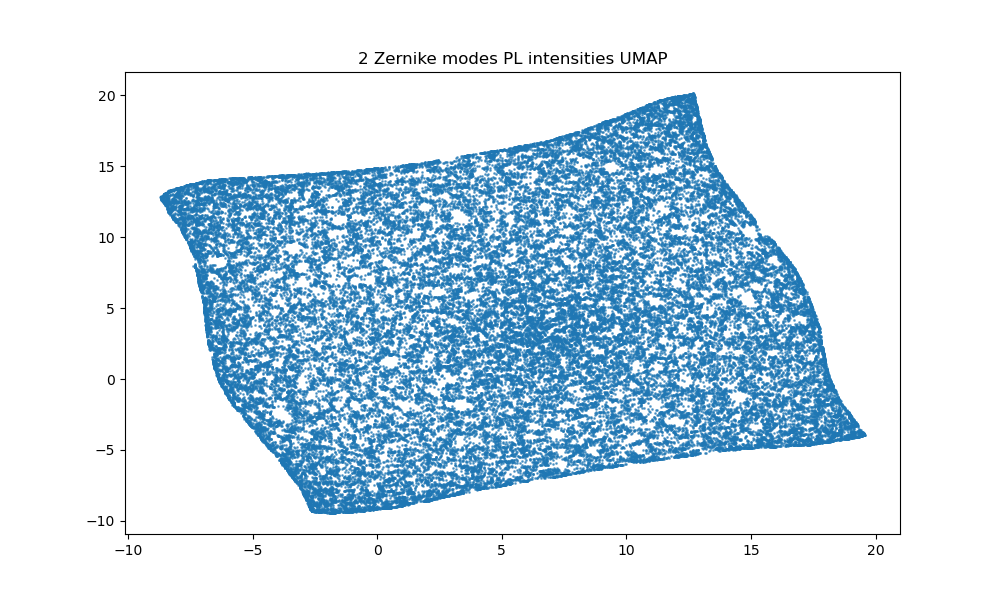
\includegraphics[ width=0.31\textwidth]{pid-2mplumap.png}}
			\hspace{\fill}
			\subfloat[2 Zernike modes PSF UMAP]{%
			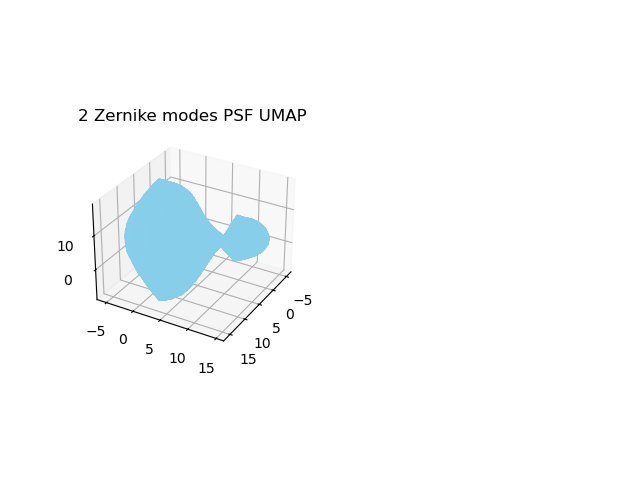
\includegraphics[ width=0.31\textwidth]{pid-2mpsfumap.png}}
			\\
			
			\subfloat[5 Zernike modes LP coefficients UMAP]{%
			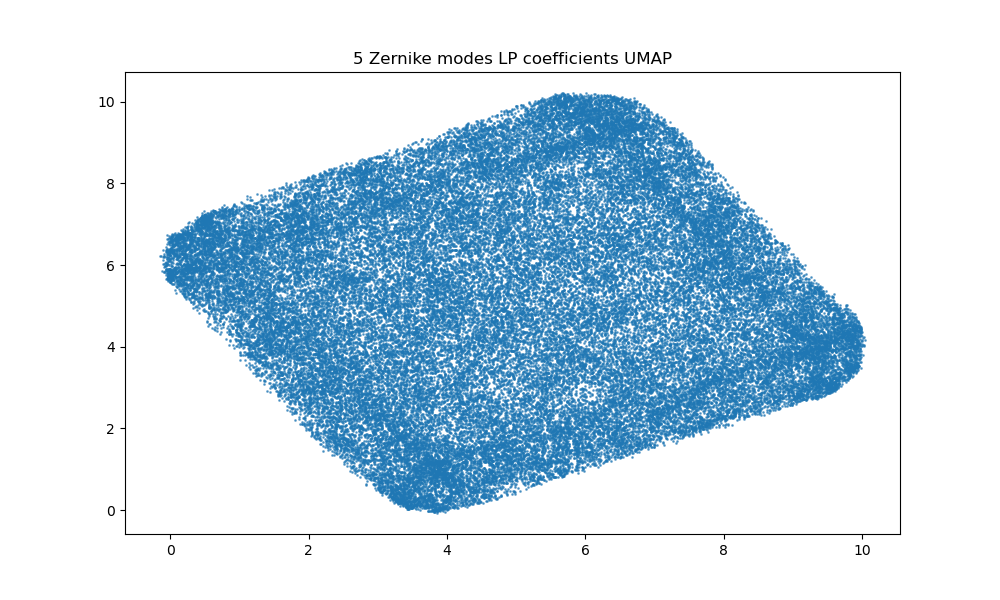
\includegraphics[ width=0.31\textwidth]{pid-5mlpumap.png}}
			\hspace{\fill}
			\subfloat[5 Zernike modes PL intensities UMAP]{%
			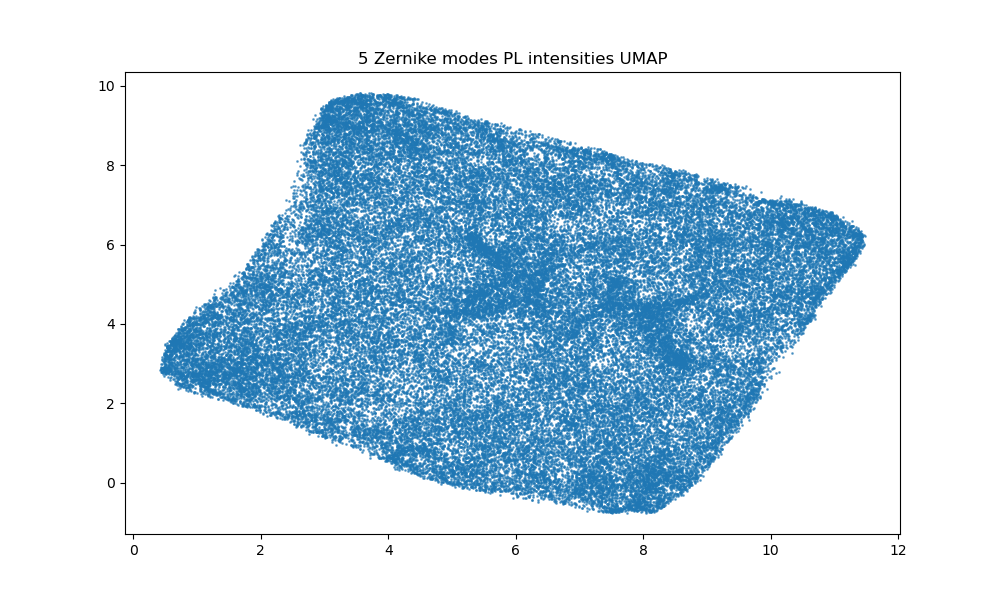
\includegraphics[ width=0.31\textwidth]{pid-5mplumap.png}}
			\hspace{\fill}
			\subfloat[5 Zernike modes PSF UMAP]{%
			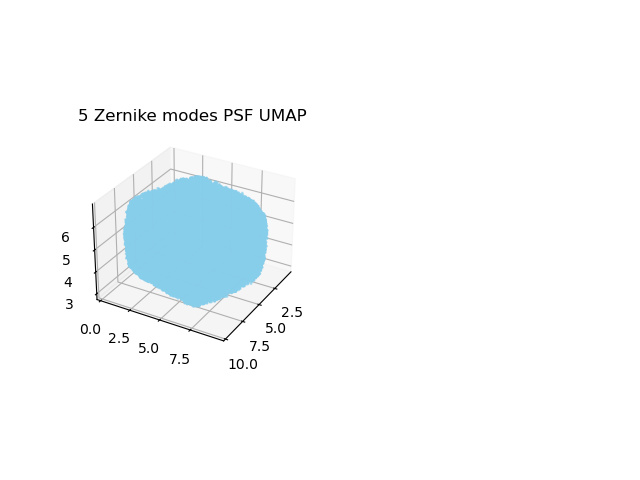
\includegraphics[ width=0.31\textwidth]{pid-5mpsfumap.png}}
			\\
			
			\subfloat[9 Zernike modes LP coefficients UMAP]{%
			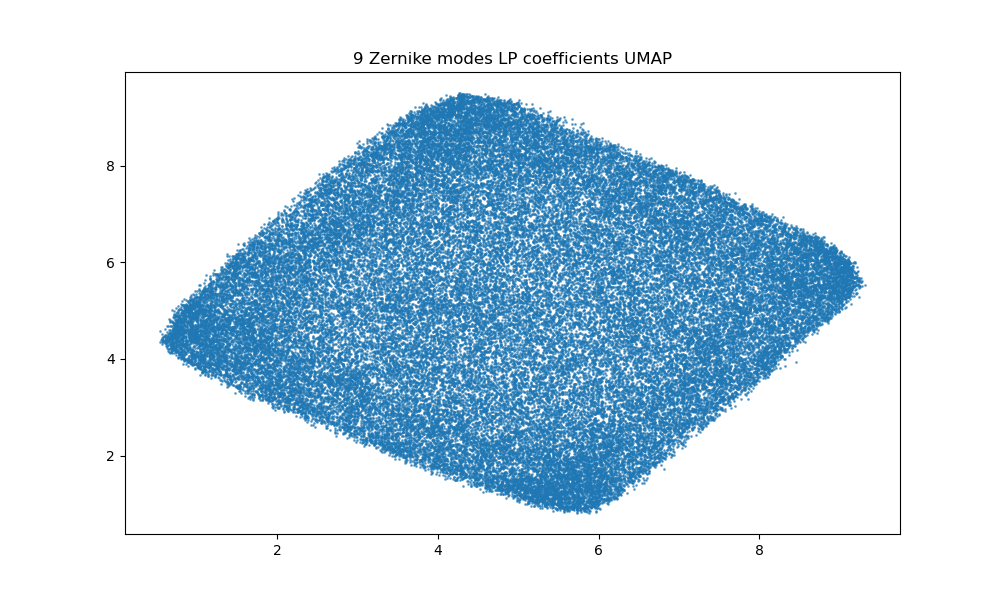
\includegraphics[ width=0.31\textwidth]{pid-9mlpumap.png}}
			\hspace{\fill}
			\subfloat[9 Zernike modes PL intensities UMAP]{%
			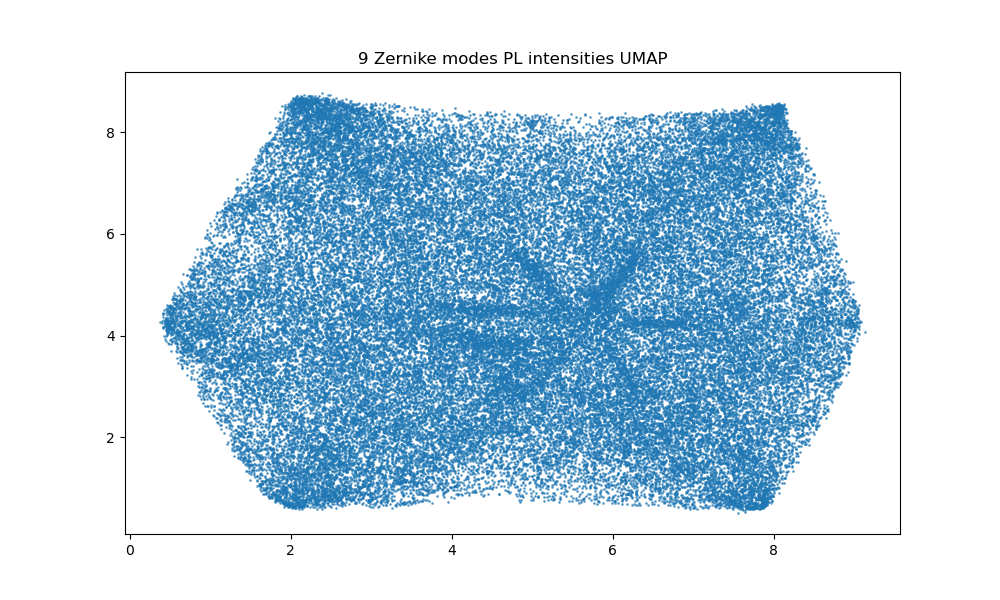
\includegraphics[ width=0.31\textwidth]{pid-9mplumap.png}}
			\hspace{\fill}
			\subfloat[9 Zernike modes PSF UMAP]{%
			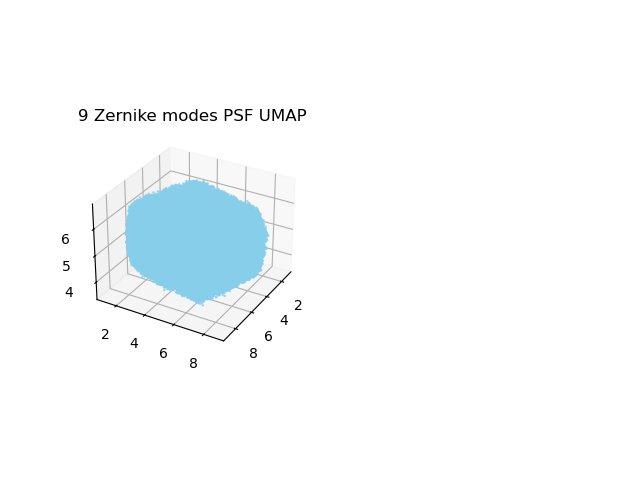
\includegraphics[ width=0.31\textwidth]{pid-9mpsfumap.png}}
			\\
			
			\subfloat[14 Zernike modes LP coefficients UMAP]{%
			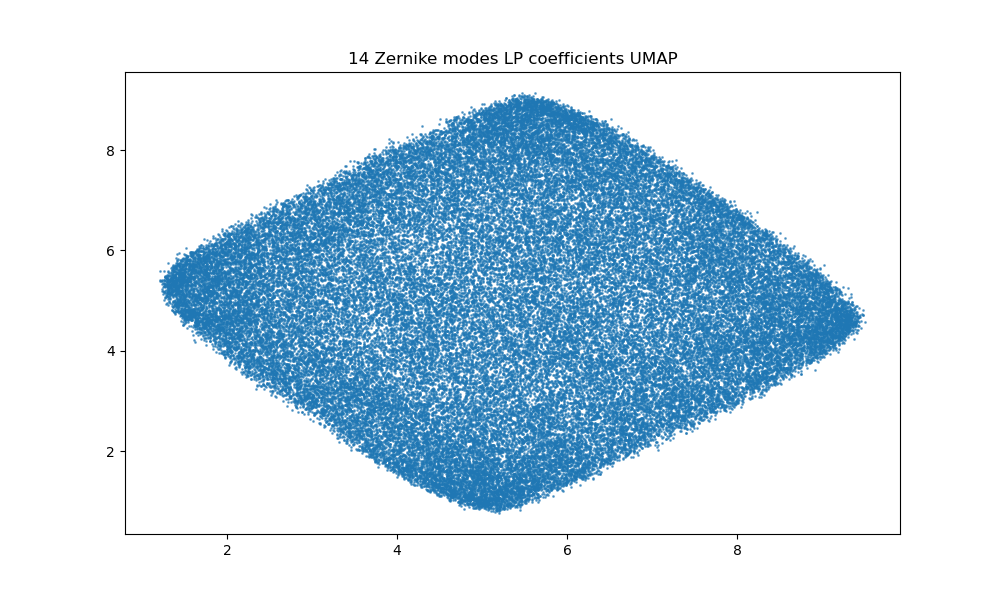
\includegraphics[ width=0.31\textwidth]{pid-14mlpumap.png}}
			\hspace{\fill}
			\subfloat[14 Zernike modes PL intensities UMAP]{%
			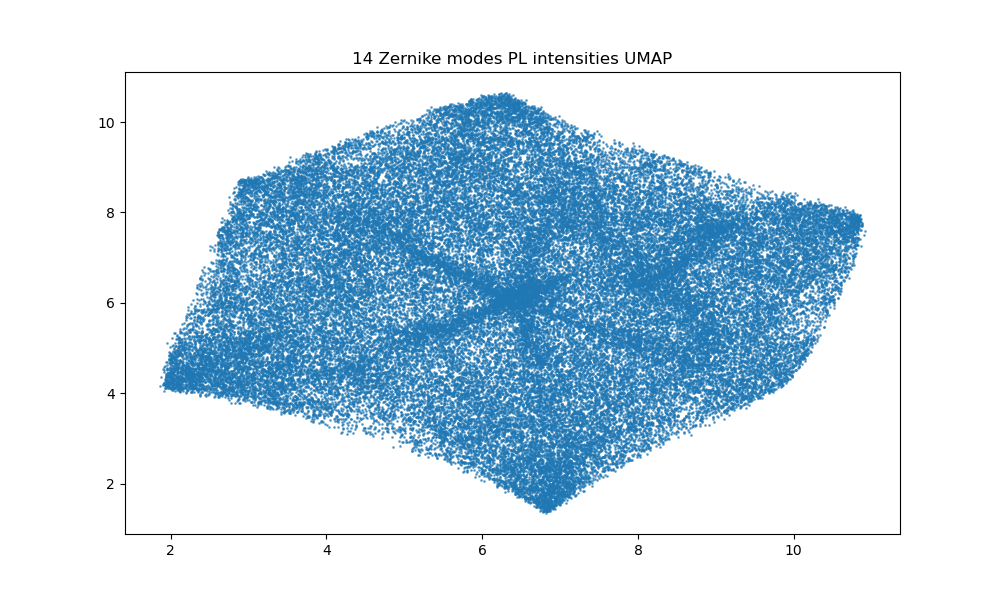
\includegraphics[ width=0.31\textwidth]{pid-14mplumap.png}}
			\hspace{\fill}
			\subfloat[14 Zernike modes PSF UMAP]{%
			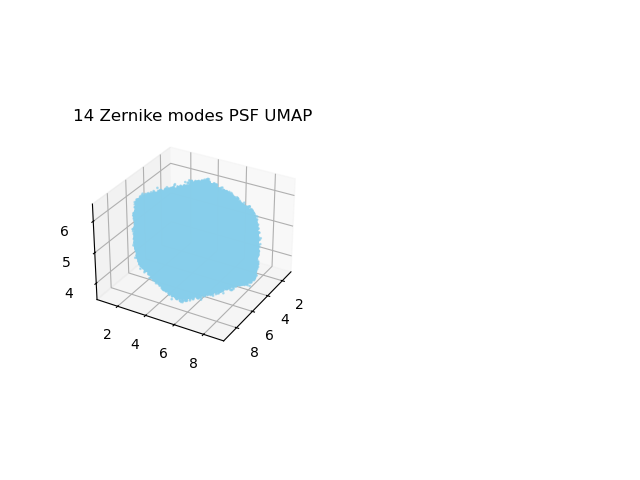
\includegraphics[ width=0.31\textwidth]{pid-14mpsfumap.png}}
			\\
			
			\subfloat[20 Zernike modes LP coefficients UMAP]{%
			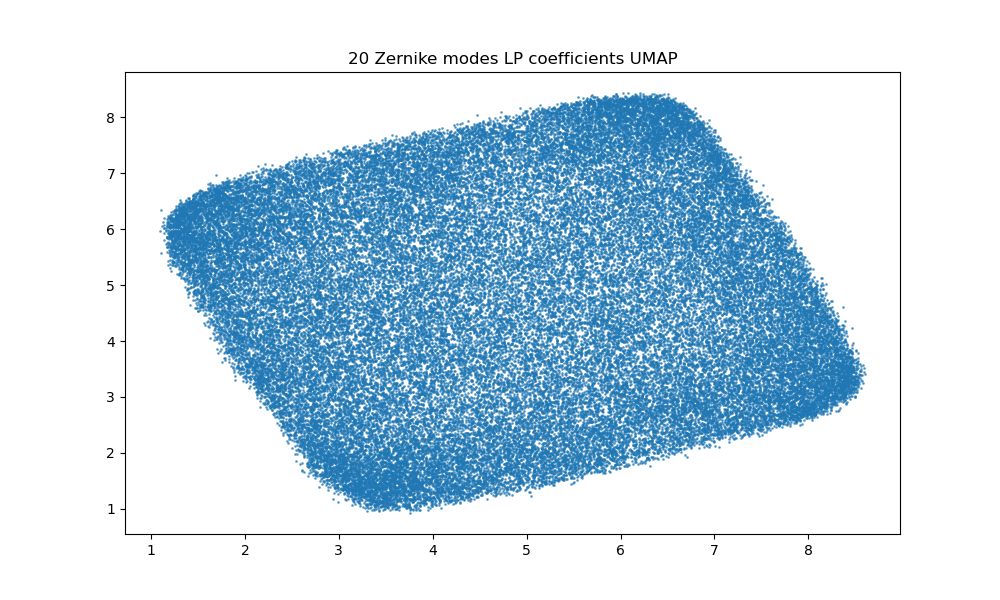
\includegraphics[ width=0.31\textwidth]{pid-20mlpumap.png}}
			\hspace{\fill}
			\subfloat[20 Zernike modes PL intensities UMAP]{%
			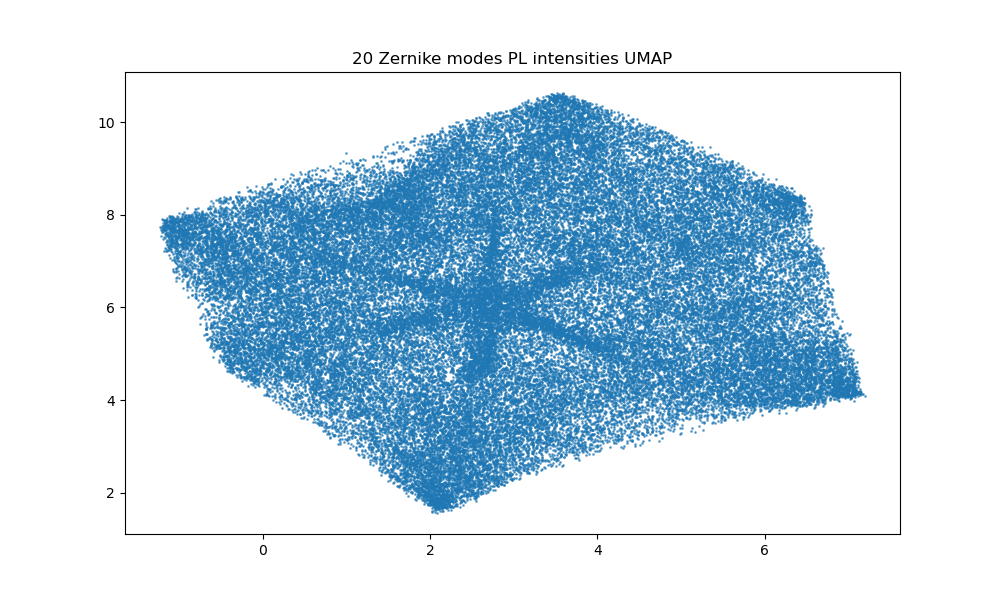
\includegraphics[ width=0.31\textwidth]{pid-20mplumap.png}}
			\hspace{\fill}
			\subfloat[20 Zernike modes PSF UMAP]{%
			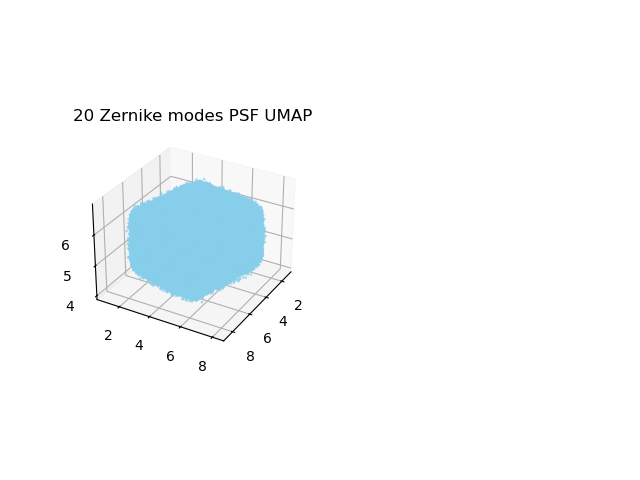
\includegraphics[ width=0.31\textwidth]{pid-20mpsfumap.png}}
			\\
			
			\caption{Datasets UMAPs}
		\end{figure*}
		\FloatBarrier
		
	
	\subsubsection{Clustering}
		
		Using DBSCAN I create clusters for the UMAP representations.
		
		\paragraph{2 Zernike modes}:
		\begin{table}[h!]
			\centering
			\begin{tabular}{|c|c|c|c|c|}
				\hline
				\textbf{} & \textbf{LP coeffs} & \textbf{PL intensities} & \textbf{PSF} & \textbf{Pred PSF}\\
				\hline
				\textbf{DBSCAN $\epsilon$} & 0.11 & 0.102 & 0.125 & 0.125\\
				\hline
				\textbf{DBSCAN neighbors} & 6 & 4 & 6 & 6\\
				\hline
				\textbf{Number of clusters} & 1447 & 1553 & 1485 & 1528\\
				\hline
				\textbf{Cluster density mean} & 42.37 & 41.59 & 41.52 & 40.20\\
				\hline
				\textbf{Cluster density variance} & 157.86 & 188.90 & 90.50 & 87.57\\
				\hline
				\textbf{Non noise points} & 61313 & 64594 & 61665 & 61427\\
				\hline
			\end{tabular}
		\caption{Clustering for 2 Zernike modes datasets}
		\end{table}
		\FloatBarrier
		
		\paragraph{5 Zernike modes}:
		\begin{table}[h!]
			\centering
			\begin{tabular}{|c|c|c|c|c|}
				\hline
				\textbf{} & \textbf{LP coeffs} & \textbf{PL intensities} & \textbf{PSF} & \textbf{Pred PSF}\\
				\hline
				\textbf{DBSCAN $\epsilon$} & 0.0385 & 0.041 & 0.131 & 0.131\\
				\hline
				\textbf{DBSCAN neighbors} & 5 & 5 & 5 & 5\\
				\hline
				\textbf{Number of clusters} & 1601 & 1527 & 1591 & 1681\\
				\hline
				\textbf{Cluster density mean} & 39.42 & 41.43 & 33.00 & 31.36\\
				\hline
				\textbf{Cluster density variance} & 348.27 & 273.60 & 857.67 & 844.99\\
				\hline
				\textbf{Non noise points} & 63120 & 63266 & 52509 & 52719\\
				\hline
			\end{tabular}
		\caption{Clustering for 5 Zernike modes datasets}
		\end{table}
		\FloatBarrier
		
		\paragraph{9 Zernike modes}:
		\begin{table}[h!]
			\centering
			\begin{tabular}{|c|c|c|c|c|}
				\hline
				\textbf{} & \textbf{LP coeffs} & \textbf{PL intensities} & \textbf{PSF} & \textbf{Pred PSF}\\
				\hline
				\textbf{DBSCAN $\epsilon$} & 0.0335 & 0.0355 & 0.105 & 0.105\\
				\hline
				\textbf{DBSCAN neighbors} & 6 & 5 & 5 & 5\\
				\hline
				\textbf{Number of clusters} & 1649 & 1666 & 1685 & 1628\\
				\hline
				\textbf{Cluster density mean} & 37.05 & 37.29 & 30.04 & 31.95\\
				\hline
				\textbf{Cluster density variance} & 239.01 & 403.49 & 843.20 & 900.53 \\
				\hline
				\textbf{Non noise points} & 61106 & 62136 & 50619 & 52024\\
				\hline
			\end{tabular}
		\caption{Clustering for 9 Zernike modes datasets}
		\end{table}
		\FloatBarrier
		
		\paragraph{14 Zernike modes}:
		\begin{table}[h!]
			\centering
			\begin{tabular}{|c|c|c|c|c|}
				\hline
				\textbf{} & \textbf{LP coeffs} & \textbf{PL intensities} & \textbf{PSF} & \textbf{Pred PSF}\\
				\hline
				\textbf{DBSCAN $\epsilon$} & 0.0322 & 0.0355 & 0.1 & 0.1\\
				\hline
				\textbf{DBSCAN neighbors} & 6 & 6 & 5 & 5\\
				\hline
				\textbf{Number of clusters} & 1472 & 1590 & 1481 & 1467\\
				\hline
				\textbf{Cluster density mean} & 41.82 & 37.57 & 36.07 & 36.30\\
				\hline
				\textbf{Cluster density variance} & 330.54 & 322.57 & 998.39 & 1013.64\\
				\hline
				\textbf{Non noise points} & 61570 & 59751 & 53428 & 53265\\
				\hline
			\end{tabular}
		\caption{Clustering for 14 Zernike modes datasets}
		\end{table}
		\FloatBarrier
		
		\paragraph{20 Zernike modes}:
		\begin{table}[h!]
			\centering
			\begin{tabular}{|c|c|c|c|c|}
				\hline
				\textbf{} & \textbf{LP coeffs} & \textbf{PL intensities} & \textbf{PSF} & \textbf{Pred PSF}\\
				\hline
				\textbf{DBSCAN $\epsilon$} & 0.031 & 0.0348 & 0.094 & 0.094\\
				\hline
				\textbf{DBSCAN neighbors} & 6 & 7 & 5 & 5\\
				\hline
				\textbf{Number of clusters} & 1596 & 1574 & 1543 & 1702\\
				\hline
				\textbf{Cluster density mean} & 38.09 & 35.22 & 33.11 & 28.75\\
				\hline
				\textbf{Cluster density variance} & 305.13 & 250.72 & 905.19 & 810.40\\
				\hline
				\textbf{Non noise points} & 60804 & 55444 & 51090 & 48941\\
				\hline
			\end{tabular}
		\caption{Clustering for 20 Zernike modes datasets}
		\end{table}
		\FloatBarrier
		
		
	\subsubsection{Normalised Mutual Information}
		
		After running an NMI on the clusters these are the results:
		\begin{lstlisting}
	NMI from datasets created with 2 Zernike Modes
    		- LP coeffs and PL intensities:
    			0.8219524719004785
    		- LP coeffs and PSF: 
    			0.8267679974838258
    		- PL intensities and PSF:
    			0.8006407078651336
    		- LP coeffs and predicted PSF: 
    			0.8278719240660488
    		- PL intensities and predicted PSF: 
    			0.8031544640644421
    		- Predicted PSF and original PSF: 
    			0.8462724838435687
    				
	NMI from datasets created with 5 Zernike Modes
    		- LP coeffs and PL intensities: 
    			0.42285255296107516
    		- LP coeffs and PSF clusters: 
    			0.3621602125646374
    		- PL intensities and PSF clusters:
    			0.26905538939513185
    		- LP coeffs and predicted PSF clusters: 
    			0.33778878770748194
    		- PL intensities and predicted PSF clusters: 
    			0.27117206275597827
    		- Predicted PSF and original PSF clusters: 
    			0.30681420233381534

	NMI from datasets created with 9 Zernike Modes
    		- LP coeffs and PL intensities: 
    			0.38776580755209583
    		- LP coeffs and PSF clusters: 
    			0.2800781281347026
    		- PL intensities and PSF clusters: 
    			0.20361911230443988
    		- LP coeffs and predicted PSF clusters: 
    			0.28157126796049103
    		- PL intensities and predicted PSF clusters: 
    			0.1996203977942372
    		- Predicted PSF and original PSF clusters: 
    			0.31825281172097275

	NMI from datasets created with 14 Zernike Modes
		- LP coeffs and PL intensities: 
			0.3384222807204235
		- LP coeffs and PSF clusters: 
			0.27310238481860455
   		- PL intensities and PSF clusters: 
   			0.18201429597315782
   		- LP coeffs and predicted PSF clusters: 
    			0.27181375146600834
    		- PL intensities and predicted PSF clusters: 
    			0.17647317929216427
    		- Predicted PSF and original PSF clusters: 
    			0.4010800021054478

	NMI from datasets created with 20 Zernike Modes
    		- LP coeffs and PL intensities:
    			0.3349100276934313
    		- LP coeffs and PSF clusters: 
    			0.2722495673325805
    		- PL intensities and PSF clusters: 
    			0.19338019736560508
    		- LP coeffs and predicted PSF clusters: 
    			0.2803220715684146
    		- PL intensities and predicted PSF clusters: 
    			0.20028997925400618
    		- Predicted PSF and original PSF clusters: 
    			0.3020698591006825
	\end{lstlisting}
	
		\begin{itemize}
			\item There is a stronger relationship between LP coefficients and PL outputs than PSF to LP coefficients.
			\item The relationship between PSF and PL outputs is the weakest.
			
		\end{itemize}		 
		\begin{figure*}[ht!]
			\centering
			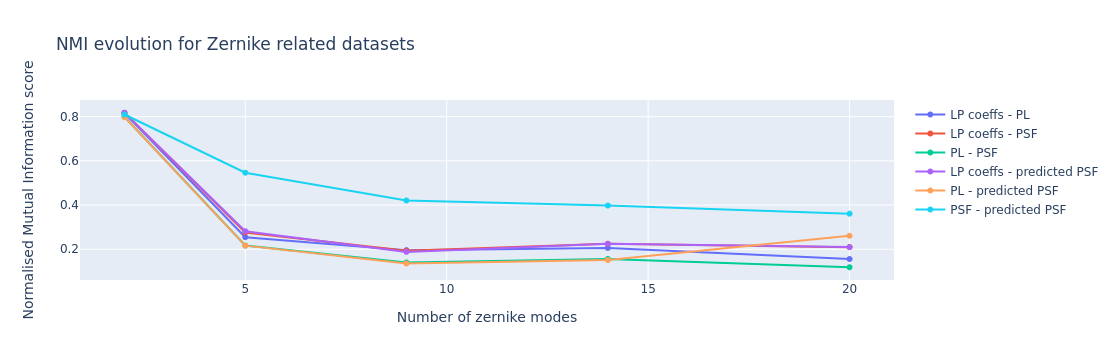
\includegraphics[width=0.7\textwidth]{pid-nmizernike.png}
			\caption{NMI evolution over Zernike related datasets}
		\end{figure*}
		
		\begin{figure*}[ht!]
			\centering
			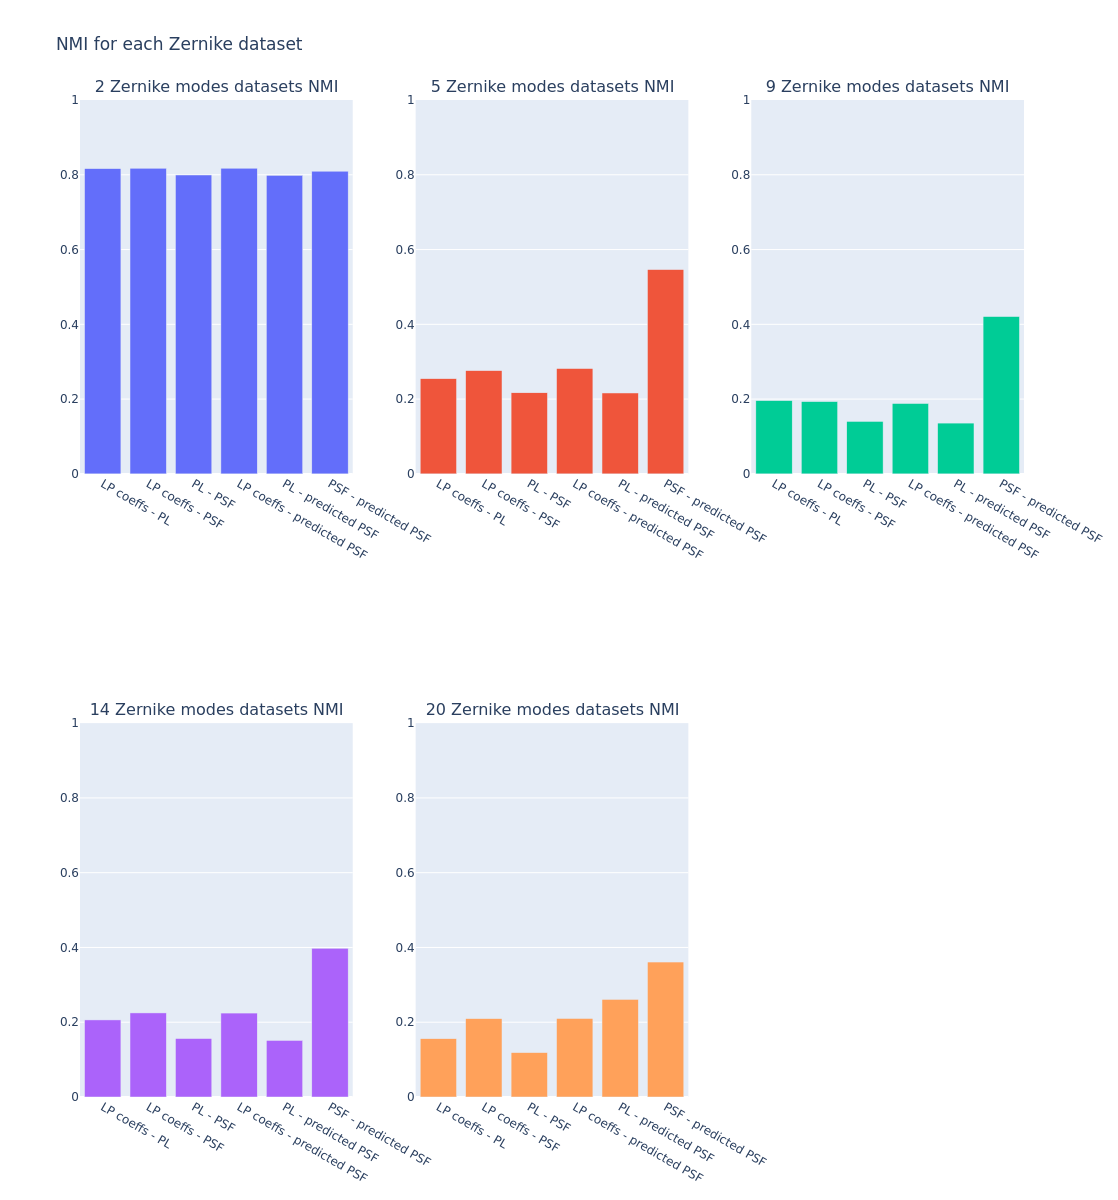
\includegraphics[width=0.7\textwidth]{pid-separatednmizernike.png}
			\caption{NMI for each of the Zernike related datasets}
		\end{figure*}